\documentclass{article}
\usepackage{algorithm}
\usepackage{algpseudocodex}
\usepackage{graphicx}
\usepackage{amsmath}
\title{CSEP521 : Applied Algorithms: Final}
\author{Karuna Sagar Krishna}

\begin{document}
    \maketitle

    \section*{Question 1}

    \subsection*{1a}
    \textbf{False}

    The question implicitly assumes that the min cut remains the same when the capacities of every edge is increased by 2. However, this is not always true as demonstrated by the graph below. Hence, as shown in the below graph, the max flow is not increased by 2 times the number of edges from $S$ to $T$ in $G$.

    Initially, the max flow was $x$ and the min cut was $S = \{s, v_0\}$ (remaining vertices in $T$). Then we increased the capacities of each edge by 2, now the max flow is $x+3$ and the min cut is $S' = \{s\}$. Clearly, the min cut has changed and the new max flow is not increased by 2 times the number of edges from $S$ to $T$

    \begin{figure}[H]
        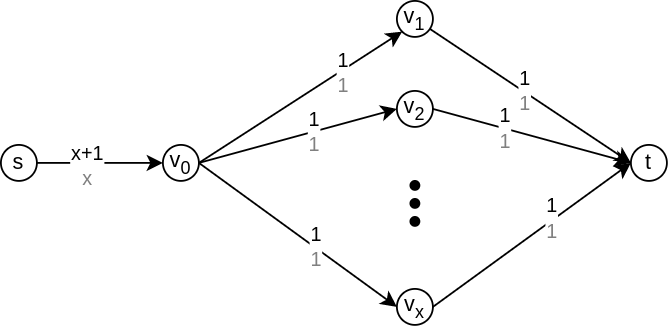
\includegraphics[width=1\textwidth]{maxflowIncreasedCapacity1.png}
    \end{figure}

    \begin{figure}[H]
        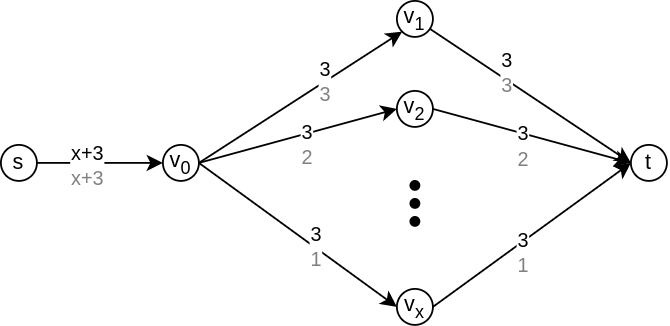
\includegraphics[width=1\textwidth]{maxflowIncreasedCapacity2.png}
    \end{figure}

    \subsection*{1b}
    \textbf{True}

    We could have a naive algorithm that iterates through all subsets of vertices checking to see if this subset covers all the edges and recording this subset if it has the minimum cardinality. There are $2^n$ subsets and each iteration takes $O(m) = O(n^2)$ time to verify if all edges are covered. Therefore, this algorithm takes $2^n + O(n^2) = 2^n$ time.

    \subsection*{1c}
    \textbf{True}

    We can compute $k = n/10$ in constant time. As clarified, we can assume that $k$ is an integer. Then the problem can be rephrased as find the $k$'th smallest number in a list of $n$ numbers, which we have solved in class in linear time.

    \subsection*{1d}
    \textbf{False}

    Applying master recurrence theorem, we get $\Theta(n^{\log_2 3})$ since $a > b^d$ i.e. $3 > 2^1$. Clearly, this does not grow the same as $\Theta(n^{\log_3 2})$

    \subsection*{1e}
    \textbf{True}

    Applying master recurrence theorem, we get $\Theta(n^2)$ since $a < b^d$ i.e. $12 < 4^2$

    \subsection*{1f}
    \textbf{False}

    As we proved in class, 3-SAT is NP complete problem. To solve any NP problem we can first spend polynomial time (by definition of NP complete) to reduce 3-SAT and then solve 3-SAT in linear time. However, the reduction is not necessarily linear hence the overall solution to any NP problem is not necessarily linear.

    \subsection*{1g}
    \textbf{False}

    In class, we discussed $EXP$ as a set of decision problems with runtime in the form $O(2^{f(n)})$ where $f(n)$ is some polynomial in input length $n$. However, there might be some decision problem with factorial complexity which grows faster than exponential functions and not part of $EXP$

    \subsection*{1h}
    \textbf{True}

    We've proved in class that every tree with $n$ vertices has exactly $n-1$ edges. Each edge contributes 2 to overall sum of degrees. So the sum of degrees across all vertices is $2(n-1)$, hence average degree per vertex is $\frac{2(n-1)}{n} = 2 - \frac{2}{n}$

    \subsection*{1i}
    \textbf{True}

    In class, we discussed why linear programs are powerful by showing that any boolean circuit can be represented as a linear program. Any instance of Program-SAT is a boolean circuit which can be converted to linear program. This conversion is mechanical and can be done in polynomial time by iterating through each line of the Program-SAT instance. Also, as we saw in class, computing the Program-SAT on a given input is equivalent to finding satisfying assignment to linear program constraints.

    \subsection*{1j}
    \textbf{True}

    Yes, as seen in class, linear programs can be solved in polynomial time using ellipsoid algorithm.

    \subsection*{1k}
    \textbf{True}

    The cut property of MST says that the minimum weight edge crossing any cut must be included in every MST. Say, $e = (u, v)$ and consider the cut formed by $\{u\}$ and $V - \{u\}$. Clearly, $e$ is the minimum weight edge crossing this cut and by cut property $e$ should be included in every MST.

    \subsection*{1l}
    \textbf{True}

    We could think of any linear program as finding the farthest point in the polytope defined by a set of inequality constraints. So if the linear program has an optimal solution, we can visualize this as a vertex on this polytope.

    \subsection*{1m}
    \textbf{False}

    Below is a counter example. Each edge in $G_3$ has capacity equal to the sum of the capacities of corresponding edge in $G_1$ and $G_2$ as indicated by the question. However, the max flow in $G_3$ is not the sum of max flow in $G_1$ and $G_2$

    \begin{figure}[H]
        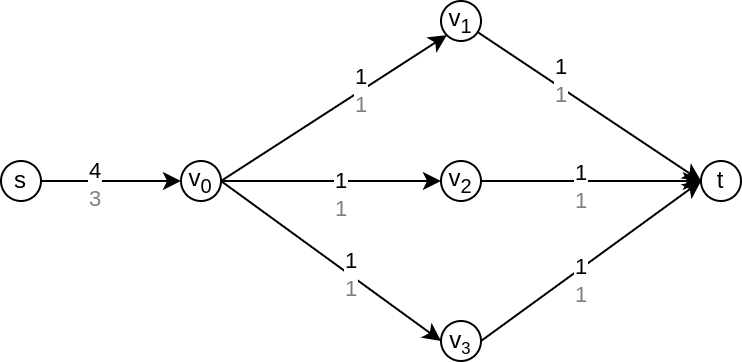
\includegraphics[width=1\textwidth]{maxflow1.png}
        \caption{$G_1$ has max flow of 3}
    \end{figure}

    \begin{figure}[H]
        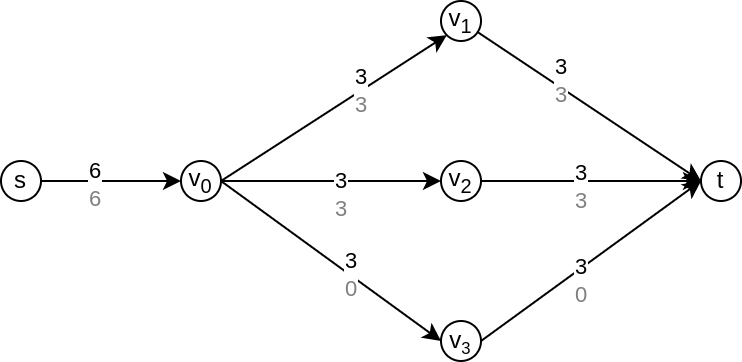
\includegraphics[width=1\textwidth]{maxflow2.png}
        \caption{$G_2$ has max flow of 6}
    \end{figure}

    \begin{figure}[H]
        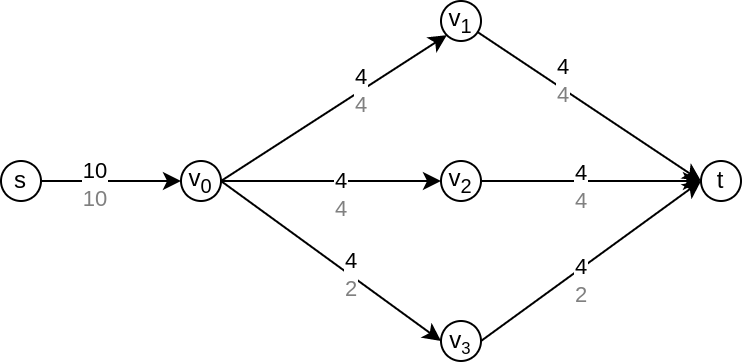
\includegraphics[width=1\textwidth]{maxflow3.png}
        \caption{$G_3$ has max flow of 10}
    \end{figure}

    \subsection*{1n}
    \textbf{True}

    We saw a greedy algorithm to find the vertex cover that is atmost twice as big as size of optimal cover. The greedy rule is to pick edge that is not covered by any vertex chosen for the cover so far. One way to implement this greedy algorithm is to iterate over edges, adding its endpoints to our vertex cover and then removing all other edges touching these endpoints. This would run in $O(n+m)$ as each edge and vertex is visited once.

    \subsection*{1o}
    \textbf{False}

    We've proved in class that, the max number of edge disjoint paths is equal to the max flow. The max flow is atmost the capacity of any cut. So it is not possible to have number of edge disjoint paths to exceed the min cut. Since the capacity of some cut (assuming unit capacity for all edges) $l$ is greater than or equal to min cut, it is not possible to have atleast $l$ edge disjoint paths.

    \subsection*{1p}
    \textbf{True}

    $f(x)$ is a decision problem to determine if $x$ is sum of squares. If we show this is in $NP$, then we can reduce this to 3-SAT in polynomial time since 3-SAT is NP complete and then solve 3-SAT in polynomial time. Hence, $f(x)$ can be solved in polynomial time.

    To prove $f(x)$ is in $NP$, we provide the following certifier that runs in polynomial time. This certifier takes the input to the decision problem $x$ and certificate $y$ and $z$ which are integers. Note, $|y| \le |x|$ and $|x| \le |x|$. The certifier performs two integer multiplications for which we learnt some fast polynomial time algorithms and one integer addition which takes linear time.

    \begin{algorithm}[H]
        \begin{algorithmic}
            \Procedure{SumOfSquaresCertifier}{$x, y, z$}
                \If{$y*y + z*z = x$}
                    \State \Return $True$
                \Else
                    \State \Return $False$
                \EndIf
            \EndProcedure
        \end{algorithmic}
    \end{algorithm}

    \subsection*{1q}
    \textbf{True}

    Bellman Ford algorithm can detect negative weight cycles. This takes $O((n+m)n)$ time. Since $m = O(n^2)$, we can say Bellman Ford takes $O((n+n^2)n) = O(n^3)$ time.

    \subsection*{1r}
    \textbf{True}

    Since both 3-SAT and vertex cover are NP complete, we can reduce vertex cover problem instances to 3-SAT in polynomial time $f(x)$. In this question, since we have a $2^{O(\log^2 n)}$ algorithm to solve 3-SAT, we can solve vertex cover in $2^{O(\log^2 n)} + f(x) = 2^{O(\log^2 n)}$ time.

    \subsection*{1s}
    \textbf{True}

    We saw Kruskal's algorithm run in $O(m \log n)$ time when implemented using union find data structure.

    \subsection*{1t}
    \textbf{True}

    Divide the $n \times n$ input matrix to form $k \times k$ matrix where each element is a matrix of size $\frac{n}{k} \times \frac{n}{k}$. We are given an algorithm that multiplies $k \times k$ matrices using $r$ multiplications and $k^2$ additions. Since each element of this $k \times k$ matrix is a subproblem of size $\frac{n}{k}$, we'll have $r$ multiplications of $\frac{n}{k} \times \frac{n}{k}$ matrices and $k^2$ additions of $\frac{n}{k} \times \frac{n}{k}$ matrices. Thus running time is $T(n) = rT(\frac{n}{k}) + k^2 (\frac{n}{k})^2$, which can be simplified as $T(n) = rT(\frac{n}{k}) + n^2$. We are also told, $3 > \log_k r > 2$ which can be rewritten as $k^3 > r > k^2$. Applying master recurrence theorem, we get $T(n) = \Theta(n^{\log_k r})$ since $a > b^d$ i.e. $r > k^2$. Hence, we can multiply $n \times n$ matrices in $O(n^{\log_k r})$

    \section*{Question 2}

    \subsection*{Idea}
    If all edges have the same cost, it doesn't matter the order in which we pick the edges. So every spanning tree is a MST. BFS can find a breadth first spanning tree in $O(n+m)$ time.
    
    However, in the question we have a graph $G$ whose edges have cost $\in \{1, 2, 3\}$. If were to apply Kruskal's algorithm, we would have sorted the edges and then picked edges in this sorted order that don't form cycle. Clearly, we would have processed all edges with cost 1 and then process all edges with cost 2 and so on. Also, Kruskal's would consider edges that connect different components to avoid cycle in spanning tree. So consider a subgraph $G_1 = (V_1, E_1)$, where $V_1 = V$ and $E_1 = \{e \in E : c(e) = 1\}$ i.e. $E_1$ only contains edges of $G$ with cost 1. Notice, $G_1$ is a graph with all edges having the same cost, hence we can run BFS to find a spanning tree. $G_1$ might be disconnected though $G$ is connected, hence BFS is run on each connected component of $G_1$. This produces a forest of spanning trees. Next, we create subgraph $G_2 = (V_2, E_2)$, where each vertex in $V_2$ represents the connected component in $G_1$ and $E_2 = \{e \in E : c(e) = 2 \land \text{$e$ connects different components}\}$. Since all edges of $G_2$ have the same cost, we can run BFS to again yield a forest of spanning trees. We repeat this and create create $G_3$ and run BFS. Since $G$ was connected, $G_3$ would be connected since it has encoded all the edges in $G$ based on how we constructed $G_3$ from $G_2$ which was inturn constructed from $G_1$. So BFS on $G_3$ should return a single spanning tree and this would the MST of $G$.
    
    \subsection*{Algorithm}
        \begin{algorithm}[H]
            \begin{algorithmic}
                \Procedure{NameTODO}{ParametersTODO}
                    \State $x = y$
                \EndProcedure
            \end{algorithmic}
        \end{algorithm}

    \subsection*{Correctness}

    \subsection*{Analysis}

    \section*{Question 3}

    \section*{Question 4}

\end{document}
 